Let $n$ be a fixed positive integer. An $n$-staircase is a polyomino with $\frac{n(n+1)}{2}$ cells arranged in the shape of a staircase, with arbitrary size. Here are two examples of $5$-staircases:

\begin{center}
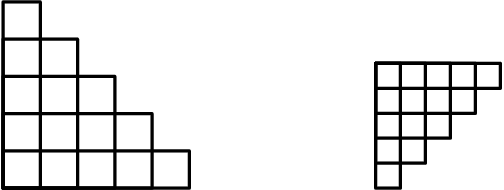
\includegraphics[width = 50.400000000000006mm]{img/fig0.png}
\end{center}
Prove that an $n$-staircase can be dissected into strictly smaller $n$-staircases.

